\section{Review of Previous Work}
\label{sec:prev}

{\bf Canonical Decision Diagrams:} 
The Reduced Ordered Binary Decision Diagram
(ROBBD) \cite{BRYA86}, based on the Shannon's decomposition, was the
first significant contribution in this area. 
Motivated by the success of BDDs, 
variants of the Shannon's decomposition principle (Davio,
Reed-Muller, etc.) were explored to develop other functional decision
diagrams: FDDs \cite{okfdd}, ADDs \cite{add}, %MTBDDs\cite{mtbdd},  
HDDs \cite{hdd} and EVBDDs \cite{evbdd}. 
%While these are %{\it curiously} still 
%referred to as {\it Word-Level Decision Diagrams} \cite{WLS}, 
Binary Moment Diagrams (BMDs) \cite{bmd}, and its derivative K*BMDs
\cite{kbmd}, % and *PHDDs \cite{phdd}, 
depart from the Boolean
decomposition and perform the decomposition of a {\it linear} function
based on its two moments. The decomposition is still point-wise,
binary, w.r.t. each Boolean variable; these do not
serve the purpose of word-level abstraction from bit-level
representations. 

%% BMDs provide a compact representation for
%% integer arithmetic circuits such as multipliers and squarers. However,
%% these are inapplicable for modulo-arithmetic circuits over Galois fields.
%in our application, we encounter modulo-arithmetic circuits and that
%too over Galois fields. For such applications, these representations
%are inapplicable. Taylor Expansion Diagrams (TEDs) \cite{ted_tcomp}
%generalize the linear moment decomposition of BMDs into a Taylor
%series expansion --- this allows the representation of RTL
%descriptions as polynomials over bit-vectors. However, 
Taylor Expansion Diagrams (TEDs) \cite{ted_tcomp} are a word-level
canonical representation of a {\it polynomial expression}, but they do
not represent a {\it polynomial function} canonically. 
%For example, $f_1 = 0$ and $f_2 = 2x^2 - 2x
%\pmod{ 4}$ are two different polynomial representations of the zero
%function over $\Z_4$; but they are symbolically different
%polynomials and they have different (non-isomorphic) TED DAGs. 
While \cite{shekhar:tcad07}  and \cite{alizadeh:tcad2010} provide
canonical representations of polynomial functions, they do so over
$\Z_{2^k}$ and not over $\Fkk$.
%finite integer rings and not over Galois fields.  


MODDs \cite{modd} \cite{modd_tcomp} are a DAG representation of the
characteristic function of a circuit over Galois fields $\Fkk$. MODDs
come very close to satisfying our requirements as a canonical
word-level representation that can be employed over Galois fields, as
it essentially interpolates a polynomial from the characteristic 
function. However, MODDs do not scale very well for large circuits ---
this is because every node in the DAG can have up to $k$ children and
the normalization operations are very complicated for MODDs. They 
suffer from the size explosion problem during intermediate
computations. They are known to be infeasible beyond
32-bit circuits.  

%In the realm of theorem-proving and SMT-solving, many automated
%decision procedures have been devised that can decide
%satisfiability/validity of word-level formulas represented by a
%combination of theories, but they do not provide a canonical
%representation of the function implemented by a ``bit-blasted''
%circuit. 

{\bf Verification of Galois field circuits:} 
%% Symbolic computer algebra techniques have been employed for formal
%% verification of circuits over $\Z_{2^k}$ and also over $\Fkk$. 
%% %% The work of \cite{gao:gf-gb-ms} shows how to use Gr\"obner basis
%% %% techniques to count the zeros of an ideal $J$ over ${\mathbb{F}}_q$
%% %% (i.e. count $V_{{\mathbb{F}}_q}(J)$). The authors then follow-up with
%% %% an approach for {\it quantifier elimination} over Galois fields
%% %% ${\mathbb{F}}_q$ \cite{gao:qe-gf-gb}. While the above works present
%% %% the theory and algorithms, efficiency/improvements in Gr\"obner basis
%% %% computation is not addressed. So is also the case with other general
%% %% verification techniques using Gr\"obner bases \cite{Avrunin:CAV}
%% %% \cite{gbverify:2007} \cite{manna:program}, etc. 
%% The paper \cite{wienand:cav08} addresses verification of
%% finite-precision integer datapath circuits using the concepts of
%% Gr\"obner bases over the ring ${\mathbb{Z}}_{2^k}$. 
%% %They model the
%% %circuit constraints by way of arithmetic-bit-level (ABL) polynomials
%% %($\{G\}$) and formulate the verification test as an equivalent
%% %{\it variety subset problem}. To solve this, first they derive a term
%% %order to represent the circuit polynomials $\{G\}$ with a Gr\"obner
%% %basis. Then they compute a normal form $f$ of the specification $g$
%% %w.r.t. $\{G\}$. They show that, under certain constraints that are
%% %satisfied by their term order, the circuit is correct if and only if
%% %$f$ is a vanishing polynomial over ${\mathbb{Z}}_{2^k}$
%% %\cite{shekhar:tcad07}. 
%% In \cite{wedler:date11}, the authors further
%% show an integration of their approach within an SMT-solver for
%% arithmetic instances.  
%% %show that  the vanishing polynomial test can be
%% %omitted by formulating the problem directly over $Q :=
%% %{\mathbb{Z}}_{2^k} [X]/\langle x^2-x : x \in X \rangle$. 
In %\cite{ibm:ecc-ita11} \cite{blueveri:ita} 
\cite{ibm:blueveri},
%from IBM needs special mention: T
the authors present the {\sc BLUEVERI} tool from IBM for verification
of Galois field circuits for error correcting codes against an
algorithmic spec. The implementation consists of a set of
(pre-designed and verified) circuit blocks that are interconnected to
form the error correcting system. The spec is given as a set of design
constraints on a ``check file''. Their objective is to prove the 
equivalence of the implementation against this check file,
%They model
%the verification instance as a data-flow graph, represent each
%sub-circuit block with its known (word-level) polynomial over $\Fq$,
%and formulate the verification problem using the {\it Weak
%  Nullstellensatz} --- i.e. to check if the {\it variety} of the
%algebraic system ``{\it spec} $\neq$ {\it implementation}'' is empty
for which they employ a Nullstellensatz formulation.
%for which they use a Gr\"obner basis engine. 
%Their main
%contributions are: i) a ``term re-writing'' to specify the algorithmic
%description using polynomials (ideal); and ii) integrating an
%AIG-style \cite{AIG:2002} Boolean solver with their word-level
%decision procedure, with lazy signal computations and Boolean
%reasoning. 
For final verification, the polynomial system is given
to a computer algebra tool ({\sc Singular} \cite{DGPS}) to {\it
  compute} a reduced Gr\"obner basis. However, improvements to the
core Gr\"obner basis computational engine are not the subject of their
work.   

In %\cite{lv:phd} 
\cite{lv:date2012} 
%\cite{lv:hldvt2011} \cite{lv:vlsi2012}, 
{\it Lv et al.} present computer algebra
techniques for formal verification of Galois field arithmetic
circuits. Given a specification polynomial $f$, and a circuit $C$,
they formulate the verification problems as an ideal membership test
using the Strong Nullstellensatz and Gr\"obner bases. In \cite{lv:date2012}, the
authors show that for any combinational circuit, {\it there exists
a term order $>_1$ that renders the set of polynomials of the circuit
itself a Gr\"obner basis --- and this term order can be easily derived
by performing a topological traversal of the circuit}. By exploiting
this term order, verification can be significantly scaled
to $163$-bit (NIST-specified) cryptography circuits. 
In contrast to the work of \cite{lv:date2012}, we are not given a
specification polynomial. Given the circuit $C$, we want
to derive (extract) the word-level specification $f$. 
In this work, we build upon the results of
%\cite{gao:gf-gb-ms} \cite{gao:qe-gf-gb} %\cite{modd_tcomp} 
\cite{lv:date2012}. 

{\bf Polynomial Interpolation in Symbolic Computation:}
The problem of polynomial interpolation is a fundamental problem in
symbolic and algebraic computing which finds application in modular
algorithms, such as the GCD computation and polynomial
factorization. The problem is stated as follows: Given $n$ distinct
data points $x_1, \dots, x_n$, and their evaluations at these points
$y_1, \dots, y_n$,  {\it interpolate} a polynomial $\F(X)$ of degree
$n-1$ (or less) such that $\F(x_i) = y_i$ for $1 \leq i \leq n$. 
Let $t$ be the number of non-zero terms in $\F$ and let $T$ be the
total number of possible terms. When ${{t} \over {T}} << 1$, the
polynomial $\F$ is {\it sparse}, otherwise it is {\it dense}. Much of
the work in polynomial interpolation addresses sparse 
interpolation using the ``black-box'' model (also called the
algebraic circuit model) as shown in Fig. \ref{fig:blackbox}. 

\begin{figure}[hbt]
\centerline{
%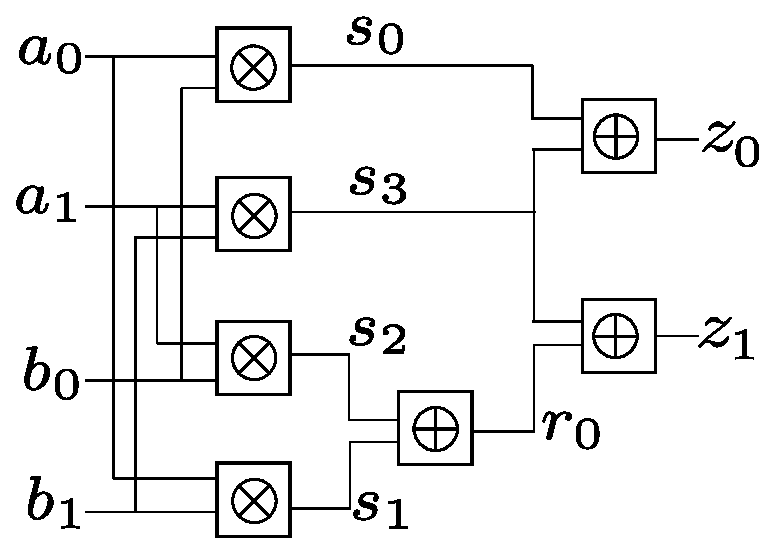
\includegraphics[scale=0.3]{../figures/2bitmultiplier.eps}
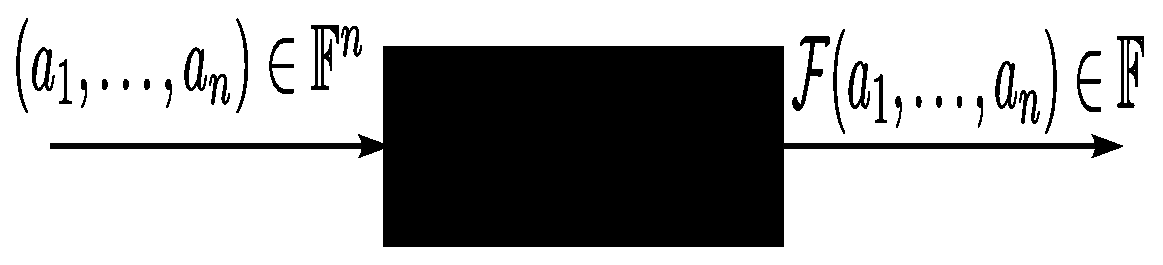
\includegraphics[scale=0.35]{../blackbox.eps}
}
\caption{The black-box or the algebraic circuit representation.}
\label{fig:blackbox}
\end{figure}

Let $\F$ be a multivariate polynomial in $n$ variables $\{x_1, \dots,
x_n\}$, with $t$ non-zero terms ($0 < t < T$), represented with a
black-box $B$. On input $(x_1, \dots, x_n)$,
the black-box evaluates $y_i = \F(x_1, \dots, x_n)$. Given also a
degree bound $d$ on $\F$, the goal is to interpolate the polynomial
$\F$ with a minimum number of {\it probes} to the black-box. The early
work of Zippel \cite{zippel:interpolate} and
Ben-Or/Tiwari \cite{ben-or-tiwari:interpolate} require $O(ndt)$ and
$O(T \log n)$ probes, respectively, to the black-box. These bounds
have since been improved significantly; the recent algorithm of
\cite{monagan:interpolate} interpolates with $O(nt)$ probes.  

Our problem falls into the category of {\it dense} interpolation, as
we require a polynomial that describes the function at each of the $q$
points of the field $\Fq$. Newton's dense interpolation technique,
with the black-box model, bounds the number of probes by $(d+1)^n$ ---
which  exhibits very high complexity. In the logic synthesis area, the
work of \cite{zilic:interpolate} investigates dense interpolation. Due
to the inherent high-complexity, their approach is feasible only for
applications over small fields, {\it e.g.} computing  Reed-Muller
forms for multi-valued logic.  

We can also employ the black-box model by replacing the black-box
(algebraic circuit) by the given circuit $C$; then every {\it probe}
of the black-box would correspond to a {\it simulation of the
  circuit}. As we desire a polynomial representation of the entire
function, exhaustive simulation would be required, which is
infeasible. Therefore, we propose a {\it symbolic approach} to
polynomial interpolation from a circuit using the Gr\"obner basis
computation. 
%It can be shown that the computational complexity of
%computing a Gr\"obner basis for our problem, in the worst case, is
%$q^{O(n)}$, where $q = 2^k$, $k$ is the datapath width and $n$ is the
%number of variables in the circuit.  
